\documentclass[twoside]{book}

% Packages required by doxygen
\usepackage{fixltx2e}
\usepackage{calc}
\usepackage{doxygen}
\usepackage[export]{adjustbox} % also loads graphicx
\usepackage{graphicx}
\usepackage[utf8]{inputenc}
\usepackage{makeidx}
\usepackage{multicol}
\usepackage{multirow}
\PassOptionsToPackage{warn}{textcomp}
\usepackage{textcomp}
\usepackage[nointegrals]{wasysym}
\usepackage[table]{xcolor}

% Font selection
\usepackage[T1]{fontenc}
\usepackage[scaled=.90]{helvet}
\usepackage{courier}
\usepackage{amssymb}
\usepackage{sectsty}
\renewcommand{\familydefault}{\sfdefault}
\allsectionsfont{%
  \fontseries{bc}\selectfont%
  \color{darkgray}%
}
\renewcommand{\DoxyLabelFont}{%
  \fontseries{bc}\selectfont%
  \color{darkgray}%
}
\newcommand{\+}{\discretionary{\mbox{\scriptsize$\hookleftarrow$}}{}{}}

% Page & text layout
\usepackage{geometry}
\geometry{%
  a4paper,%
  top=2.5cm,%
  bottom=2.5cm,%
  left=2.5cm,%
  right=2.5cm%
}
\tolerance=750
\hfuzz=15pt
\hbadness=750
\setlength{\emergencystretch}{15pt}
\setlength{\parindent}{0cm}
\setlength{\parskip}{3ex plus 2ex minus 2ex}
\makeatletter
\renewcommand{\paragraph}{%
  \@startsection{paragraph}{4}{0ex}{-1.0ex}{1.0ex}{%
    \normalfont\normalsize\bfseries\SS@parafont%
  }%
}
\renewcommand{\subparagraph}{%
  \@startsection{subparagraph}{5}{0ex}{-1.0ex}{1.0ex}{%
    \normalfont\normalsize\bfseries\SS@subparafont%
  }%
}
\makeatother

% Headers & footers
\usepackage{fancyhdr}
\pagestyle{fancyplain}
\fancyhead[LE]{\fancyplain{}{\bfseries\thepage}}
\fancyhead[CE]{\fancyplain{}{}}
\fancyhead[RE]{\fancyplain{}{\bfseries\leftmark}}
\fancyhead[LO]{\fancyplain{}{\bfseries\rightmark}}
\fancyhead[CO]{\fancyplain{}{}}
\fancyhead[RO]{\fancyplain{}{\bfseries\thepage}}
\fancyfoot[LE]{\fancyplain{}{}}
\fancyfoot[CE]{\fancyplain{}{}}
\fancyfoot[RE]{\fancyplain{}{\bfseries\scriptsize Generated by Doxygen }}
\fancyfoot[LO]{\fancyplain{}{\bfseries\scriptsize Generated by Doxygen }}
\fancyfoot[CO]{\fancyplain{}{}}
\fancyfoot[RO]{\fancyplain{}{}}
\renewcommand{\footrulewidth}{0.4pt}
\renewcommand{\chaptermark}[1]{%
  \markboth{#1}{}%
}
\renewcommand{\sectionmark}[1]{%
  \markright{\thesection\ #1}%
}

% Indices & bibliography
\usepackage{natbib}
\usepackage[titles]{tocloft}
\setcounter{tocdepth}{3}
\setcounter{secnumdepth}{5}
\makeindex

% Hyperlinks (required, but should be loaded last)
\usepackage{ifpdf}
\ifpdf
  \usepackage[pdftex,pagebackref=true]{hyperref}
\else
  \usepackage[ps2pdf,pagebackref=true]{hyperref}
\fi
\hypersetup{%
  colorlinks=true,%
  linkcolor=blue,%
  citecolor=blue,%
  unicode%
}

% Custom commands
\newcommand{\clearemptydoublepage}{%
  \newpage{\pagestyle{empty}\cleardoublepage}%
}

\usepackage{caption}
\captionsetup{labelsep=space,justification=centering,font={bf},singlelinecheck=off,skip=4pt,position=top}

%===== C O N T E N T S =====

\begin{document}

% Titlepage & ToC
\hypersetup{pageanchor=false,
             bookmarksnumbered=true,
             pdfencoding=unicode
            }
\pagenumbering{alph}
\begin{titlepage}
\vspace*{7cm}
\begin{center}%
{\Large rt2\+\_\+ass2 \\[1ex]\large 1.\+0 }\\
\vspace*{1cm}
{\large Generated by Doxygen 1.8.13}\\
\end{center}
\end{titlepage}
\clearemptydoublepage
\pagenumbering{roman}
\tableofcontents
\clearemptydoublepage
\pagenumbering{arabic}
\hypersetup{pageanchor=true}

%--- Begin generated contents ---
\chapter{rt2\+\_\+ass2}
\label{md__r_e_a_d_m_e}
\Hypertarget{md__r_e_a_d_m_e}
Second and final assignment of the Research Track 2 course 
\chapter{Namespace Index}
\section{Namespace List}
Here is a list of all documented namespaces with brief descriptions\+:\begin{DoxyCompactList}
\item\contentsline{section}{\hyperlink{namespacego__to__point__action}{go\+\_\+to\+\_\+point\+\_\+action} }{\pageref{namespacego__to__point__action}}{}
\end{DoxyCompactList}

\chapter{File Index}
\doxysection{File List}
Here is a list of all documented files with brief descriptions\+:\begin{DoxyCompactList}
\item\contentsline{section}{scripts/\mbox{\hyperlink{go__to__point__action_8py}{go\+\_\+to\+\_\+point\+\_\+action.\+py}} \\*This file will directly operate on the robot based on the goal received }{\pageref{go__to__point__action_8py}}{}
\item\contentsline{section}{src/\mbox{\hyperlink{position__service_8cpp}{position\+\_\+service.\+cpp}} \\*This file will generate a service to require random x,y,theta values }{\pageref{position__service_8cpp}}{}
\item\contentsline{section}{src/\mbox{\hyperlink{state__machine_8cpp}{state\+\_\+machine.\+cpp}} \\*This file will let the user interface comunicate with the \mbox{\hyperlink{namespacego__to__point__action}{go\+\_\+to\+\_\+point\+\_\+action}} }{\pageref{state__machine_8cpp}}{}
\end{DoxyCompactList}

\chapter{Namespace Documentation}
\hypertarget{namespacego__to__point__action}{}\doxysection{go\+\_\+to\+\_\+point\+\_\+action Namespace Reference}
\label{namespacego__to__point__action}\index{go\_to\_point\_action@{go\_to\_point\_action}}
\doxysubsection*{Functions}
\begin{DoxyCompactItemize}
\item 
def \mbox{\hyperlink{namespacego__to__point__action_affe1389e38557b69ee71adea85b846b2}{clbk\+\_\+odom}} (msg)
\begin{DoxyCompactList}\small\item\em The clbk\+\_\+odom function. \end{DoxyCompactList}\item 
def \mbox{\hyperlink{namespacego__to__point__action_ab7ad2629ed9ffbd5d9b7ca9c540d932a}{change\+\_\+state}} (state)
\begin{DoxyCompactList}\small\item\em The change\+\_\+state function. \end{DoxyCompactList}\item 
def \mbox{\hyperlink{namespacego__to__point__action_a0bca87c6d45ca63d3152a4e8def72e2a}{normalize\+\_\+angle}} (angle)
\begin{DoxyCompactList}\small\item\em The normalize\+\_\+angle function. \end{DoxyCompactList}\item 
def \mbox{\hyperlink{namespacego__to__point__action_a18e7fef09d30f59bb91061f4b91f87e6}{fix\+\_\+yaw}} (des\+\_\+pos)
\begin{DoxyCompactList}\small\item\em The fix\+\_\+yah function. \end{DoxyCompactList}\item 
def \mbox{\hyperlink{namespacego__to__point__action_a7c35034eab524fbff7d05d80fd65ede4}{go\+\_\+straight\+\_\+ahead}} (des\+\_\+pos)
\begin{DoxyCompactList}\small\item\em The go\+\_\+straight\+\_\+ahead function. \end{DoxyCompactList}\item 
def \mbox{\hyperlink{namespacego__to__point__action_a068188471dd5fc0ed3ea371e3a32338a}{fix\+\_\+final\+\_\+yaw}} (des\+\_\+yaw)
\begin{DoxyCompactList}\small\item\em The fix\+\_\+final\+\_\+yah function. \end{DoxyCompactList}\item 
def \mbox{\hyperlink{namespacego__to__point__action_a9fec1cd57aebd720828b5bab962048db}{done}} ()
\begin{DoxyCompactList}\small\item\em The done function. \end{DoxyCompactList}\item 
def \mbox{\hyperlink{namespacego__to__point__action_ab3bc8cf3239eaa0def69f3a87a98976c}{planning}} (goal)
\begin{DoxyCompactList}\small\item\em The planning function. \end{DoxyCompactList}\item 
def \mbox{\hyperlink{namespacego__to__point__action_a33cfc08b34e07f53ddda67d2ab551ba1}{main}} ()
\begin{DoxyCompactList}\small\item\em Documentation for the main function. \end{DoxyCompactList}\end{DoxyCompactItemize}
\doxysubsection*{Variables}
\begin{DoxyCompactItemize}
\item 
\mbox{\Hypertarget{namespacego__to__point__action_afd83e8a50982500cb1aea028fa6bd8fb}\label{namespacego__to__point__action_afd83e8a50982500cb1aea028fa6bd8fb}} 
{\bfseries position\+\_\+} = Point()
\item 
\mbox{\Hypertarget{namespacego__to__point__action_a7e81c61a8a01745a08f175577455bcb4}\label{namespacego__to__point__action_a7e81c61a8a01745a08f175577455bcb4}} 
int {\bfseries yaw\+\_\+} = 0
\item 
\mbox{\Hypertarget{namespacego__to__point__action_a513d83133bce80caeaf1f02289d6c12b}\label{namespacego__to__point__action_a513d83133bce80caeaf1f02289d6c12b}} 
int {\bfseries state\+\_\+} = 0
\item 
\mbox{\Hypertarget{namespacego__to__point__action_a6d09e37099932459bc3e4146007cce86}\label{namespacego__to__point__action_a6d09e37099932459bc3e4146007cce86}} 
{\bfseries pub\+\_\+} = None
\item 
\mbox{\Hypertarget{namespacego__to__point__action_a99d0c1c8c5e359fcd5f1901e25a86a2d}\label{namespacego__to__point__action_a99d0c1c8c5e359fcd5f1901e25a86a2d}} 
int {\bfseries yaw\+\_\+precision\+\_\+} = math.\+pi / 9
\item 
\mbox{\Hypertarget{namespacego__to__point__action_aeaede468f4753c2c476474b35b81754c}\label{namespacego__to__point__action_aeaede468f4753c2c476474b35b81754c}} 
int {\bfseries yaw\+\_\+precision\+\_\+2\+\_\+} = math.\+pi / 90
\item 
\mbox{\Hypertarget{namespacego__to__point__action_a01a3cd0c013f3c1712758e04b4bc91f4}\label{namespacego__to__point__action_a01a3cd0c013f3c1712758e04b4bc91f4}} 
float {\bfseries dist\+\_\+precision\+\_\+} = 0.\+1
\item 
\mbox{\Hypertarget{namespacego__to__point__action_a67a9de26fa4f88312f9cc4a8ecedb369}\label{namespacego__to__point__action_a67a9de26fa4f88312f9cc4a8ecedb369}} 
float {\bfseries kp\+\_\+a} = -\/3.\+0
\item 
\mbox{\Hypertarget{namespacego__to__point__action_acd565e807f177f678d6a12d504d01e60}\label{namespacego__to__point__action_acd565e807f177f678d6a12d504d01e60}} 
float {\bfseries kp\+\_\+d} = 0.\+2
\item 
\mbox{\Hypertarget{namespacego__to__point__action_a9cb07d74a9d8087eb04da488c77c118c}\label{namespacego__to__point__action_a9cb07d74a9d8087eb04da488c77c118c}} 
float {\bfseries ub\+\_\+a} = 0.\+6
\item 
\mbox{\Hypertarget{namespacego__to__point__action_a156fcdad5d5c28042b46d45d323a9fac}\label{namespacego__to__point__action_a156fcdad5d5c28042b46d45d323a9fac}} 
float {\bfseries lb\+\_\+a} = -\/0.\+5
\item 
\mbox{\Hypertarget{namespacego__to__point__action_a05a9d1a5cc9bd5e985d6ad5247ac985d}\label{namespacego__to__point__action_a05a9d1a5cc9bd5e985d6ad5247ac985d}} 
float {\bfseries ub\+\_\+d} = 0.\+6
\item 
\mbox{\Hypertarget{namespacego__to__point__action_a3994b1577d1a499ce8c7352036ee6486}\label{namespacego__to__point__action_a3994b1577d1a499ce8c7352036ee6486}} 
{\bfseries act\+\_\+s} = None
\end{DoxyCompactItemize}


\doxysubsection{Detailed Description}
\begin{DoxyVerb}.. module:: go_to_point_action
   :platform: Unix
   :synopsis: Python module for piloting the robot to the target

.. moduleauthor:: Carmine Recchiuto <carmine.recchiuto@dibris.unige.it>

ROS node for driving a robot to a specific point

Subscribes to:
    /odom topic where the simulator publishes the robot position

Publishes to:
    /cmd_vel the desired robot position

Service :
    /go_to_point to start the robot motion.
\end{DoxyVerb}
 

\doxysubsection{Function Documentation}
\mbox{\Hypertarget{namespacego__to__point__action_ab7ad2629ed9ffbd5d9b7ca9c540d932a}\label{namespacego__to__point__action_ab7ad2629ed9ffbd5d9b7ca9c540d932a}} 
\index{go\_to\_point\_action@{go\_to\_point\_action}!change\_state@{change\_state}}
\index{change\_state@{change\_state}!go\_to\_point\_action@{go\_to\_point\_action}}
\doxysubsubsection{\texorpdfstring{change\_state()}{change\_state()}}
{\footnotesize\ttfamily def go\+\_\+to\+\_\+point\+\_\+action.\+change\+\_\+state (\begin{DoxyParamCaption}\item[{}]{state }\end{DoxyParamCaption})}



The change\+\_\+state function. 

It controls the state of the robot, allowing to translate or to rotate when needed. \mbox{\Hypertarget{namespacego__to__point__action_affe1389e38557b69ee71adea85b846b2}\label{namespacego__to__point__action_affe1389e38557b69ee71adea85b846b2}} 
\index{go\_to\_point\_action@{go\_to\_point\_action}!clbk\_odom@{clbk\_odom}}
\index{clbk\_odom@{clbk\_odom}!go\_to\_point\_action@{go\_to\_point\_action}}
\doxysubsubsection{\texorpdfstring{clbk\_odom()}{clbk\_odom()}}
{\footnotesize\ttfamily def go\+\_\+to\+\_\+point\+\_\+action.\+clbk\+\_\+odom (\begin{DoxyParamCaption}\item[{}]{msg }\end{DoxyParamCaption})}



The clbk\+\_\+odom function. 

This Callback is for the subscriber to topic odom it keeps track of the robot pose.

\begin{DoxyItemize}
\item msg the message carrying the information \end{DoxyItemize}
\mbox{\Hypertarget{namespacego__to__point__action_a9fec1cd57aebd720828b5bab962048db}\label{namespacego__to__point__action_a9fec1cd57aebd720828b5bab962048db}} 
\index{go\_to\_point\_action@{go\_to\_point\_action}!done@{done}}
\index{done@{done}!go\_to\_point\_action@{go\_to\_point\_action}}
\doxysubsubsection{\texorpdfstring{done()}{done()}}
{\footnotesize\ttfamily def go\+\_\+to\+\_\+point\+\_\+action.\+done (\begin{DoxyParamCaption}{ }\end{DoxyParamCaption})}



The done function. 

It stops the robot meaning that the pose has been reached \mbox{\Hypertarget{namespacego__to__point__action_a068188471dd5fc0ed3ea371e3a32338a}\label{namespacego__to__point__action_a068188471dd5fc0ed3ea371e3a32338a}} 
\index{go\_to\_point\_action@{go\_to\_point\_action}!fix\_final\_yaw@{fix\_final\_yaw}}
\index{fix\_final\_yaw@{fix\_final\_yaw}!go\_to\_point\_action@{go\_to\_point\_action}}
\doxysubsubsection{\texorpdfstring{fix\_final\_yaw()}{fix\_final\_yaw()}}
{\footnotesize\ttfamily def go\+\_\+to\+\_\+point\+\_\+action.\+fix\+\_\+final\+\_\+yaw (\begin{DoxyParamCaption}\item[{}]{des\+\_\+yaw }\end{DoxyParamCaption})}



The fix\+\_\+final\+\_\+yah function. 

It allows the robot to fix it\textquotesingle{}s yah and reach the final state(done) if the conditions are met \mbox{\Hypertarget{namespacego__to__point__action_a18e7fef09d30f59bb91061f4b91f87e6}\label{namespacego__to__point__action_a18e7fef09d30f59bb91061f4b91f87e6}} 
\index{go\_to\_point\_action@{go\_to\_point\_action}!fix\_yaw@{fix\_yaw}}
\index{fix\_yaw@{fix\_yaw}!go\_to\_point\_action@{go\_to\_point\_action}}
\doxysubsubsection{\texorpdfstring{fix\_yaw()}{fix\_yaw()}}
{\footnotesize\ttfamily def go\+\_\+to\+\_\+point\+\_\+action.\+fix\+\_\+yaw (\begin{DoxyParamCaption}\item[{}]{des\+\_\+pos }\end{DoxyParamCaption})}



The fix\+\_\+yah function. 

It rotates the robot to fix it\textquotesingle{}s yah in the desired direction by publishing a twist message on /cmd\+\_\+vel 
\begin{DoxyParams}{Parameters}
{\em des\+\_\+pos} & from this desired position computes the desired yah \\
\hline
\end{DoxyParams}
\mbox{\Hypertarget{namespacego__to__point__action_a7c35034eab524fbff7d05d80fd65ede4}\label{namespacego__to__point__action_a7c35034eab524fbff7d05d80fd65ede4}} 
\index{go\_to\_point\_action@{go\_to\_point\_action}!go\_straight\_ahead@{go\_straight\_ahead}}
\index{go\_straight\_ahead@{go\_straight\_ahead}!go\_to\_point\_action@{go\_to\_point\_action}}
\doxysubsubsection{\texorpdfstring{go\_straight\_ahead()}{go\_straight\_ahead()}}
{\footnotesize\ttfamily def go\+\_\+to\+\_\+point\+\_\+action.\+go\+\_\+straight\+\_\+ahead (\begin{DoxyParamCaption}\item[{}]{des\+\_\+pos }\end{DoxyParamCaption})}



The go\+\_\+straight\+\_\+ahead function. 

It allows the robot to go straight or to change it\textquotesingle{}s state if needed \mbox{\Hypertarget{namespacego__to__point__action_a33cfc08b34e07f53ddda67d2ab551ba1}\label{namespacego__to__point__action_a33cfc08b34e07f53ddda67d2ab551ba1}} 
\index{go\_to\_point\_action@{go\_to\_point\_action}!main@{main}}
\index{main@{main}!go\_to\_point\_action@{go\_to\_point\_action}}
\doxysubsubsection{\texorpdfstring{main()}{main()}}
{\footnotesize\ttfamily def go\+\_\+to\+\_\+point\+\_\+action.\+main (\begin{DoxyParamCaption}{ }\end{DoxyParamCaption})}



Documentation for the main function. 

More details.


\begin{DoxyParams}{Parameters}
{\em None} & \\
\hline
\end{DoxyParams}
\mbox{\Hypertarget{namespacego__to__point__action_a0bca87c6d45ca63d3152a4e8def72e2a}\label{namespacego__to__point__action_a0bca87c6d45ca63d3152a4e8def72e2a}} 
\index{go\_to\_point\_action@{go\_to\_point\_action}!normalize\_angle@{normalize\_angle}}
\index{normalize\_angle@{normalize\_angle}!go\_to\_point\_action@{go\_to\_point\_action}}
\doxysubsubsection{\texorpdfstring{normalize\_angle()}{normalize\_angle()}}
{\footnotesize\ttfamily def go\+\_\+to\+\_\+point\+\_\+action.\+normalize\+\_\+angle (\begin{DoxyParamCaption}\item[{}]{angle }\end{DoxyParamCaption})}



The normalize\+\_\+angle function. 

It performs normalazation of an angle . \mbox{\Hypertarget{namespacego__to__point__action_ab3bc8cf3239eaa0def69f3a87a98976c}\label{namespacego__to__point__action_ab3bc8cf3239eaa0def69f3a87a98976c}} 
\index{go\_to\_point\_action@{go\_to\_point\_action}!planning@{planning}}
\index{planning@{planning}!go\_to\_point\_action@{go\_to\_point\_action}}
\doxysubsubsection{\texorpdfstring{planning()}{planning()}}
{\footnotesize\ttfamily def go\+\_\+to\+\_\+point\+\_\+action.\+planning (\begin{DoxyParamCaption}\item[{}]{goal }\end{DoxyParamCaption})}



The planning function. 

It is the action callback. The script will remain inside this function, due to the while loop. Here it will wait for new goal, ask the robot to reach them and delete goal if required. The state will also be updated 
\begin{DoxyParams}{Parameters}
{\em goal} & It is the goal required in the action server \\
\hline
\end{DoxyParams}

\chapter{File Documentation}
\hypertarget{go__to__point__action_8py}{}\section{scripts/go\+\_\+to\+\_\+point\+\_\+action.py File Reference}
\label{go__to__point__action_8py}\index{scripts/go\+\_\+to\+\_\+point\+\_\+action.\+py@{scripts/go\+\_\+to\+\_\+point\+\_\+action.\+py}}


This file will directly operate on the robot based on the goal received.  


\subsection*{Namespaces}
\begin{DoxyCompactItemize}
\item 
 \hyperlink{namespacego__to__point__action}{go\+\_\+to\+\_\+point\+\_\+action}
\end{DoxyCompactItemize}
\subsection*{Functions}
\begin{DoxyCompactItemize}
\item 
def \hyperlink{namespacego__to__point__action_affe1389e38557b69ee71adea85b846b2}{go\+\_\+to\+\_\+point\+\_\+action.\+clbk\+\_\+odom} (msg)
\begin{DoxyCompactList}\small\item\em The clbk\+\_\+odom function. \end{DoxyCompactList}\item 
def \hyperlink{namespacego__to__point__action_ab7ad2629ed9ffbd5d9b7ca9c540d932a}{go\+\_\+to\+\_\+point\+\_\+action.\+change\+\_\+state} (state)
\begin{DoxyCompactList}\small\item\em The change\+\_\+state function. \end{DoxyCompactList}\item 
def \hyperlink{namespacego__to__point__action_a0bca87c6d45ca63d3152a4e8def72e2a}{go\+\_\+to\+\_\+point\+\_\+action.\+normalize\+\_\+angle} (angle)
\begin{DoxyCompactList}\small\item\em The normalize\+\_\+angle function. \end{DoxyCompactList}\item 
def \hyperlink{namespacego__to__point__action_a18e7fef09d30f59bb91061f4b91f87e6}{go\+\_\+to\+\_\+point\+\_\+action.\+fix\+\_\+yaw} (des\+\_\+pos)
\begin{DoxyCompactList}\small\item\em The fix\+\_\+yah function. \end{DoxyCompactList}\item 
def \hyperlink{namespacego__to__point__action_a7c35034eab524fbff7d05d80fd65ede4}{go\+\_\+to\+\_\+point\+\_\+action.\+go\+\_\+straight\+\_\+ahead} (des\+\_\+pos)
\begin{DoxyCompactList}\small\item\em The go\+\_\+straight\+\_\+ahead function. \end{DoxyCompactList}\item 
def \hyperlink{namespacego__to__point__action_a068188471dd5fc0ed3ea371e3a32338a}{go\+\_\+to\+\_\+point\+\_\+action.\+fix\+\_\+final\+\_\+yaw} (des\+\_\+yaw)
\begin{DoxyCompactList}\small\item\em The fix\+\_\+final\+\_\+yah function. \end{DoxyCompactList}\item 
def \hyperlink{namespacego__to__point__action_a9fec1cd57aebd720828b5bab962048db}{go\+\_\+to\+\_\+point\+\_\+action.\+done} ()
\begin{DoxyCompactList}\small\item\em The done function. \end{DoxyCompactList}\item 
def \hyperlink{namespacego__to__point__action_ab3bc8cf3239eaa0def69f3a87a98976c}{go\+\_\+to\+\_\+point\+\_\+action.\+planning} (goal)
\begin{DoxyCompactList}\small\item\em The planning function. \end{DoxyCompactList}\item 
def \hyperlink{namespacego__to__point__action_a33cfc08b34e07f53ddda67d2ab551ba1}{go\+\_\+to\+\_\+point\+\_\+action.\+main} ()
\begin{DoxyCompactList}\small\item\em Documentation for the main function. \end{DoxyCompactList}\end{DoxyCompactItemize}
\subsection*{Variables}
\begin{DoxyCompactItemize}
\item 
\mbox{\Hypertarget{namespacego__to__point__action_afd83e8a50982500cb1aea028fa6bd8fb}\label{namespacego__to__point__action_afd83e8a50982500cb1aea028fa6bd8fb}} 
{\bfseries go\+\_\+to\+\_\+point\+\_\+action.\+position\+\_\+} = Point()
\item 
\mbox{\Hypertarget{namespacego__to__point__action_a7e81c61a8a01745a08f175577455bcb4}\label{namespacego__to__point__action_a7e81c61a8a01745a08f175577455bcb4}} 
int {\bfseries go\+\_\+to\+\_\+point\+\_\+action.\+yaw\+\_\+} = 0
\item 
\mbox{\Hypertarget{namespacego__to__point__action_a513d83133bce80caeaf1f02289d6c12b}\label{namespacego__to__point__action_a513d83133bce80caeaf1f02289d6c12b}} 
int {\bfseries go\+\_\+to\+\_\+point\+\_\+action.\+state\+\_\+} = 0
\item 
\mbox{\Hypertarget{namespacego__to__point__action_a6d09e37099932459bc3e4146007cce86}\label{namespacego__to__point__action_a6d09e37099932459bc3e4146007cce86}} 
{\bfseries go\+\_\+to\+\_\+point\+\_\+action.\+pub\+\_\+} = None
\item 
\mbox{\Hypertarget{namespacego__to__point__action_a99d0c1c8c5e359fcd5f1901e25a86a2d}\label{namespacego__to__point__action_a99d0c1c8c5e359fcd5f1901e25a86a2d}} 
int {\bfseries go\+\_\+to\+\_\+point\+\_\+action.\+yaw\+\_\+precision\+\_\+} = math.\+pi / 9
\item 
\mbox{\Hypertarget{namespacego__to__point__action_aeaede468f4753c2c476474b35b81754c}\label{namespacego__to__point__action_aeaede468f4753c2c476474b35b81754c}} 
int {\bfseries go\+\_\+to\+\_\+point\+\_\+action.\+yaw\+\_\+precision\+\_\+2\+\_\+} = math.\+pi / 90
\item 
\mbox{\Hypertarget{namespacego__to__point__action_a01a3cd0c013f3c1712758e04b4bc91f4}\label{namespacego__to__point__action_a01a3cd0c013f3c1712758e04b4bc91f4}} 
float {\bfseries go\+\_\+to\+\_\+point\+\_\+action.\+dist\+\_\+precision\+\_\+} = 0.\+1
\item 
\mbox{\Hypertarget{namespacego__to__point__action_a67a9de26fa4f88312f9cc4a8ecedb369}\label{namespacego__to__point__action_a67a9de26fa4f88312f9cc4a8ecedb369}} 
float {\bfseries go\+\_\+to\+\_\+point\+\_\+action.\+kp\+\_\+a} = -\/3.\+0
\item 
\mbox{\Hypertarget{namespacego__to__point__action_acd565e807f177f678d6a12d504d01e60}\label{namespacego__to__point__action_acd565e807f177f678d6a12d504d01e60}} 
float {\bfseries go\+\_\+to\+\_\+point\+\_\+action.\+kp\+\_\+d} = 0.\+2
\item 
\mbox{\Hypertarget{namespacego__to__point__action_a9cb07d74a9d8087eb04da488c77c118c}\label{namespacego__to__point__action_a9cb07d74a9d8087eb04da488c77c118c}} 
float {\bfseries go\+\_\+to\+\_\+point\+\_\+action.\+ub\+\_\+a} = 0.\+6
\item 
\mbox{\Hypertarget{namespacego__to__point__action_a156fcdad5d5c28042b46d45d323a9fac}\label{namespacego__to__point__action_a156fcdad5d5c28042b46d45d323a9fac}} 
float {\bfseries go\+\_\+to\+\_\+point\+\_\+action.\+lb\+\_\+a} = -\/0.\+5
\item 
\mbox{\Hypertarget{namespacego__to__point__action_a05a9d1a5cc9bd5e985d6ad5247ac985d}\label{namespacego__to__point__action_a05a9d1a5cc9bd5e985d6ad5247ac985d}} 
float {\bfseries go\+\_\+to\+\_\+point\+\_\+action.\+ub\+\_\+d} = 0.\+6
\item 
\mbox{\Hypertarget{namespacego__to__point__action_a3994b1577d1a499ce8c7352036ee6486}\label{namespacego__to__point__action_a3994b1577d1a499ce8c7352036ee6486}} 
{\bfseries go\+\_\+to\+\_\+point\+\_\+action.\+act\+\_\+s} = None
\end{DoxyCompactItemize}


\subsection{Detailed Description}
This file will directly operate on the robot based on the goal received. 

\begin{DoxyAuthor}{Author}
Federico Zecchi 
\end{DoxyAuthor}
\begin{DoxyDate}{Date}
18/06/21
\end{DoxyDate}
Action Server\+:~\newline
 °/go\+\_\+to\+\_\+point\+\_\+action 
\hypertarget{position__service_8cpp}{}\section{src/position\+\_\+service.cpp File Reference}
\label{position__service_8cpp}\index{src/position\+\_\+service.\+cpp@{src/position\+\_\+service.\+cpp}}


This file will generate a service to require random x,y,theta values.  


{\ttfamily \#include \char`\"{}ros/ros.\+h\char`\"{}}\newline
{\ttfamily \#include \char`\"{}rt2\+\_\+ass2/\+Random\+Position.\+h\char`\"{}}\newline
Include dependency graph for position\+\_\+service.\+cpp\+:\nopagebreak
\begin{figure}[H]
\begin{center}
\leavevmode
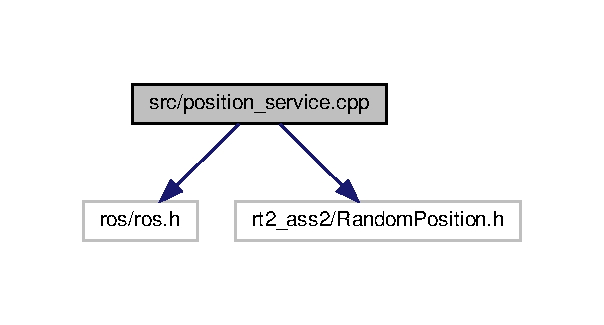
\includegraphics[width=290pt]{position__service_8cpp__incl}
\end{center}
\end{figure}
\subsection*{Functions}
\begin{DoxyCompactItemize}
\item 
double \hyperlink{position__service_8cpp_a10f83119b77a8fbd085a5550955f85ff}{rand\+M\+ToN} (double M, double N)
\item 
bool \hyperlink{position__service_8cpp_a50b96db7340f22ccfd1b065a5e159c7c}{myrandom} (rt2\+\_\+ass2\+::\+Random\+Position\+::\+Request \&req, rt2\+\_\+ass2\+::\+Random\+Position\+::\+Response \&res)
\item 
int \hyperlink{position__service_8cpp_a3c04138a5bfe5d72780bb7e82a18e627}{main} (int argc, char $\ast$$\ast$argv)
\end{DoxyCompactItemize}


\subsection{Detailed Description}
This file will generate a service to require random x,y,theta values. 

\begin{DoxyAuthor}{Author}
Federico Zecchi 
\end{DoxyAuthor}
\begin{DoxyVersion}{Version}
1 
\end{DoxyVersion}
\begin{DoxyDate}{Date}
18/06/21 
\end{DoxyDate}

\begin{DoxyParams}[1]{Parameters}
\mbox{\tt in}  & {\em world\+\_\+width} & Define the width of the discretized world\\
\hline
\end{DoxyParams}
Services\+:~\newline
 °/position\+\_\+server

Description \+:

This node will create a server to require random x,y,theta values 

\subsection{Function Documentation}
\mbox{\Hypertarget{position__service_8cpp_a3c04138a5bfe5d72780bb7e82a18e627}\label{position__service_8cpp_a3c04138a5bfe5d72780bb7e82a18e627}} 
\index{position\+\_\+service.\+cpp@{position\+\_\+service.\+cpp}!main@{main}}
\index{main@{main}!position\+\_\+service.\+cpp@{position\+\_\+service.\+cpp}}
\subsubsection{\texorpdfstring{main()}{main()}}
{\footnotesize\ttfamily int main (\begin{DoxyParamCaption}\item[{int}]{argc,  }\item[{char $\ast$$\ast$}]{argv }\end{DoxyParamCaption})}

The Main function It simply initializes the service server, binding him to its function \mbox{\Hypertarget{position__service_8cpp_a50b96db7340f22ccfd1b065a5e159c7c}\label{position__service_8cpp_a50b96db7340f22ccfd1b065a5e159c7c}} 
\index{position\+\_\+service.\+cpp@{position\+\_\+service.\+cpp}!myrandom@{myrandom}}
\index{myrandom@{myrandom}!position\+\_\+service.\+cpp@{position\+\_\+service.\+cpp}}
\subsubsection{\texorpdfstring{myrandom()}{myrandom()}}
{\footnotesize\ttfamily bool myrandom (\begin{DoxyParamCaption}\item[{rt2\+\_\+ass2\+::\+Random\+Position\+::\+Request \&}]{req,  }\item[{rt2\+\_\+ass2\+::\+Random\+Position\+::\+Response \&}]{res }\end{DoxyParamCaption})}

This function is the callback of the service /position\+\_\+server 
\begin{DoxyParams}{Parameters}
{\em req} & the request received\+: it gets two intervals of values for x and y \\
\hline
{\em res} & the response returned to the client\+: the random coordinates within a specific interval \\
\hline
\end{DoxyParams}
\mbox{\Hypertarget{position__service_8cpp_a10f83119b77a8fbd085a5550955f85ff}\label{position__service_8cpp_a10f83119b77a8fbd085a5550955f85ff}} 
\index{position\+\_\+service.\+cpp@{position\+\_\+service.\+cpp}!rand\+M\+ToN@{rand\+M\+ToN}}
\index{rand\+M\+ToN@{rand\+M\+ToN}!position\+\_\+service.\+cpp@{position\+\_\+service.\+cpp}}
\subsubsection{\texorpdfstring{rand\+M\+To\+N()}{randMToN()}}
{\footnotesize\ttfamily double rand\+M\+ToN (\begin{DoxyParamCaption}\item[{double}]{M,  }\item[{double}]{N }\end{DoxyParamCaption})}

The rand\+M\+ToN function return a random number in a certain range 
\begin{DoxyParams}{Parameters}
{\em M} & the minimum of a certain range \\
\hline
{\em N} & the maximum of a certain range \\
\hline
\end{DoxyParams}

\hypertarget{state__machine_8cpp}{}\doxysection{src/state\+\_\+machine.cpp File Reference}
\label{state__machine_8cpp}\index{src/state\_machine.cpp@{src/state\_machine.cpp}}


This file will let the user interface comunicate with the \mbox{\hyperlink{namespacego__to__point__action}{go\+\_\+to\+\_\+point\+\_\+action}}.  


{\ttfamily \#include \char`\"{}ros/ros.\+h\char`\"{}}\newline
{\ttfamily \#include \char`\"{}rt2\+\_\+ass2/\+Command.\+h\char`\"{}}\newline
{\ttfamily \#include \char`\"{}rt2\+\_\+ass2/\+Position.\+h\char`\"{}}\newline
{\ttfamily \#include \char`\"{}rt2\+\_\+ass2/\+Random\+Position.\+h\char`\"{}}\newline
{\ttfamily \#include \char`\"{}rt2\+\_\+ass2/go\+\_\+to\+\_\+point\+Action.\+h\char`\"{}}\newline
{\ttfamily \#include $<$actionlib/client/simple\+\_\+action\+\_\+client.\+h$>$}\newline
Include dependency graph for state\+\_\+machine.\+cpp\+:\nopagebreak
\begin{figure}[H]
\begin{center}
\leavevmode
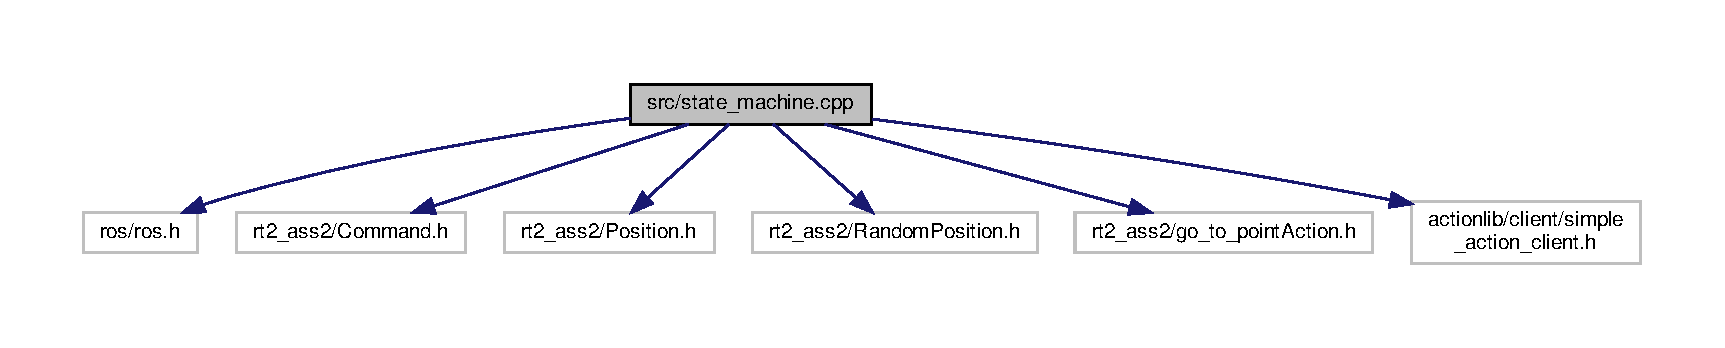
\includegraphics[width=350pt]{state__machine_8cpp__incl}
\end{center}
\end{figure}
\doxysubsection*{Functions}
\begin{DoxyCompactItemize}
\item 
bool \mbox{\hyperlink{state__machine_8cpp_ac04c316253aedc174376e609ca84098e}{user\+\_\+interface}} (rt2\+\_\+ass2\+::\+Command\+::\+Request \&req, rt2\+\_\+ass2\+::\+Command\+::\+Response \&res)
\item 
int \mbox{\hyperlink{state__machine_8cpp_a3c04138a5bfe5d72780bb7e82a18e627}{main}} (int argc, char $\ast$$\ast$argv)
\end{DoxyCompactItemize}
\doxysubsection*{Variables}
\begin{DoxyCompactItemize}
\item 
\mbox{\Hypertarget{state__machine_8cpp_aa90516c0d0bcfb73be3cb5baf2e889c6}\label{state__machine_8cpp_aa90516c0d0bcfb73be3cb5baf2e889c6}} 
bool {\bfseries send\+\_\+goal} = false
\item 
\mbox{\Hypertarget{state__machine_8cpp_a028d5a1ebf6347bef506d0f712dbea00}\label{state__machine_8cpp_a028d5a1ebf6347bef506d0f712dbea00}} 
bool {\bfseries stop\+\_\+goal} =false
\item 
\mbox{\Hypertarget{state__machine_8cpp_ab376b87f96a574a793c03c53e75afec8}\label{state__machine_8cpp_ab376b87f96a574a793c03c53e75afec8}} 
bool {\bfseries start} =false
\item 
\mbox{\Hypertarget{state__machine_8cpp_a57dccd06a6ac28217e5dda6009c4eb55}\label{state__machine_8cpp_a57dccd06a6ac28217e5dda6009c4eb55}} 
float {\bfseries lin\+\_\+vel} =0
\item 
\mbox{\Hypertarget{state__machine_8cpp_ac4793035b5d8c1967e0c092d55e5d5df}\label{state__machine_8cpp_ac4793035b5d8c1967e0c092d55e5d5df}} 
float {\bfseries ang\+\_\+vel} =0
\end{DoxyCompactItemize}


\doxysubsection{Detailed Description}
This file will let the user interface comunicate with the \mbox{\hyperlink{namespacego__to__point__action}{go\+\_\+to\+\_\+point\+\_\+action}}. 

\begin{DoxyAuthor}{Author}
Federico Zecchi 
\end{DoxyAuthor}
\begin{DoxyVersion}{Version}
1 
\end{DoxyVersion}
\begin{DoxyDate}{Date}
18/06/21 
\end{DoxyDate}

\begin{DoxyParams}[1]{Parameters}
\mbox{\texttt{ in}}  & {\em world\+\_\+width} & Define the width of the discretized world\\
\hline
\end{DoxyParams}
Services\+:~\newline
 °/user\+\_\+interface

Clients\+:~\newline
 °/position\+\_\+server

Action Client\+:~\newline
 °/go\+\_\+to\+\_\+point\+\_\+action Description \+:

This node will be the bridge between the user interface, and the \mbox{\hyperlink{namespacego__to__point__action}{go\+\_\+to\+\_\+point\+\_\+action}}. It will receive commands from the user interface. It can elaborate new random target from the position\+\_\+server. It can start or stop the \mbox{\hyperlink{namespacego__to__point__action}{go\+\_\+to\+\_\+point\+\_\+action}} 

\doxysubsection{Function Documentation}
\mbox{\Hypertarget{state__machine_8cpp_a3c04138a5bfe5d72780bb7e82a18e627}\label{state__machine_8cpp_a3c04138a5bfe5d72780bb7e82a18e627}} 
\index{state\_machine.cpp@{state\_machine.cpp}!main@{main}}
\index{main@{main}!state\_machine.cpp@{state\_machine.cpp}}
\doxysubsubsection{\texorpdfstring{main()}{main()}}
{\footnotesize\ttfamily int main (\begin{DoxyParamCaption}\item[{int}]{argc,  }\item[{char $\ast$$\ast$}]{argv }\end{DoxyParamCaption})}

The main funtion

This function initializes everithing that is needed waits for commands and then performes the various requests to services and action \mbox{\Hypertarget{state__machine_8cpp_ac04c316253aedc174376e609ca84098e}\label{state__machine_8cpp_ac04c316253aedc174376e609ca84098e}} 
\index{state\_machine.cpp@{state\_machine.cpp}!user\_interface@{user\_interface}}
\index{user\_interface@{user\_interface}!state\_machine.cpp@{state\_machine.cpp}}
\doxysubsubsection{\texorpdfstring{user\_interface()}{user\_interface()}}
{\footnotesize\ttfamily bool user\+\_\+interface (\begin{DoxyParamCaption}\item[{rt2\+\_\+ass2\+::\+Command\+::\+Request \&}]{req,  }\item[{rt2\+\_\+ass2\+::\+Command\+::\+Response \&}]{res }\end{DoxyParamCaption})}

The user\+\_\+interface function

This function is the callback function for the server of /user\+\_\+interface service 
\begin{DoxyParams}{Parameters}
{\em req} & the request received from the client of the user\+\_\+interface.\+py. \\
\hline
{\em res} & the response has not been used \\
\hline
\end{DoxyParams}

\begin{DoxyRetVals}{Return values}
{\em A} & boolean value \\
\hline
\end{DoxyRetVals}

%--- End generated contents ---

% Index
\backmatter
\newpage
\phantomsection
\clearemptydoublepage
\addcontentsline{toc}{chapter}{Index}
\printindex

\end{document}
